\documentclass{ctexart}

% --- 导入所需宏包 ---
\usepackage[a4paper, vmargin=2.5cm, hmargin=2cm]{geometry}
\usepackage{amsmath, amssymb, amsthm}
\usepackage[svgnames]{xcolor}
\usepackage[most]{tcolorbox}
\usepackage{fancyhdr}
\usepackage{lmodern} % 提供更多字体变体,包括粗斜体无衬线字体
\usepackage{tikz}
\usetikzlibrary{intersections, patterns, shadows, decorations.pathmorphing}
\usepackage{fontawesome5} % 更新的图标包
\usepackage{enumitem}
\usepackage{mdframed}
\usepackage{varwidth} % 用于varwidth环境
\usepackage{background} % 用于添加水印
\usepackage{setspace} % 用于调整行距
\usepackage{float} % 用于控制浮动体位置

% --- 修复页眉高度警告 ---
\setlength{\headheight}{22pt}

% --- 水印设置 ---
\backgroundsetup{
    scale=1,
    color=black,
    opacity=0.08,
    angle=0,
    position=current page.center,
    vshift=0cm,
    hshift=0cm,
    contents={
        \begin{tikzpicture}[remember picture, overlay]
            % 中央大水印 - 30度倾斜
            \node[rotate=30, text opacity=0.12, text=gray!40] at (0,0) 
                {\fontsize{80}{96}\selectfont\sffamily\bfseries 雪履千山客};
        \end{tikzpicture}
    }
}

% --- 自定义优雅颜色定义 ---
\definecolor{themeblue}{RGB}{52, 73, 94}%主题蓝
\definecolor{elegantpurple}{RGB}{155, 89, 182}%优雅紫
\definecolor{warmorange}{RGB}{230, 126, 34}%温暖橙
\definecolor{forestgreen}{RGB}{39, 174, 96}%森林绿
\definecolor{deepblue}{RGB}{41, 128, 185}%深邃蓝
\definecolor{sunsityellow}{RGB}{241, 196, 15}%阳光黄
\definecolor{lightgrayblue}{RGB}{236, 240, 241}%浅灰蓝
\definecolor{softpink}{RGB}{250, 219, 216}%柔和粉
\definecolor{crimsonred}{RGB}{220, 20, 60}%深红
\definecolor{darkslategray}{RGB}{47, 79, 79}%深石板灰
\definecolor{notegreen}{RGB}{39, 174, 96}%注意绿

% --- 页面布局与页眉页脚设置 ---
\pagestyle{fancy}
\fancyhf{}
\fancyhead[L]{\color{crimsonred}\textit{\faBook\ High School Mathematics Handout }}
\fancyhead[R]{\color{crimsonred}\textit{雪履千山客 \faUser}}
\fancyfoot[C]{\color{crimsonred!70}\small\textbf{--\ \thepage\ --}}
\renewcommand{\headrulewidth}{1pt}
\renewcommand{\footrulewidth}{0pt}
\renewcommand{\headrule}{\hbox to\headwidth{\color{crimsonred!30}\leaders\hrule height \headrulewidth\hfill}}

% --- 自定义优美的文本框环境 ---

% 主标题框 (斜体英文+中文,专业设计)
\newtcolorbox{chaptertitle}[3][]{
    enhanced,
    colback=themeblue!8!white,
    colframe=white,
    boxrule=0pt,
    arc=0pt,
    outer arc=0pt,
    width=0.90\textwidth,
    fonttitle=\Huge\sffamily,
    title={\makebox[1.8em][l]{\textcolor{themeblue}{#2}}\ \textbf{\textit{{#3}}}},
    coltitle=themeblue,
    center title,
    toptitle=0pt,
    bottomtitle=0pt,
    before skip=0pt,
    after skip=0pt,
    overlay={%
        \ifx\relax#1\relax\else
        \node[anchor=south east, text=themeblue!60, font=\large\itshape\kaishu, inner sep=2pt] 
            at ([xshift=-8mm,yshift=5mm]frame.south east) {\fcolorbox{white}{white!90}{\makebox[0pt][r]{#1}}};
        \fi
    }
}

% 习题框 (专业方正设计,左侧竖线,优化对齐)
\newtcolorbox{examplebox}{
    enhanced,
    colback=forestgreen!5!white,
    colframe=white,
    boxrule=0pt,
    arc=0pt,
    outer arc=0pt,
    fonttitle=\bfseries\sffamily,
    title={\makebox[1.8em][l]{\textcolor{forestgreen}{\faEdit}}\ \textit{\textcolor{white}{Example}}},
    coltitle=forestgreen!90!white,
    colbacktitle=forestgreen!35!white,
    attach boxed title to top left={yshift=-2mm, xshift=3mm},
    boxed title style={arc=0pt, outer arc=0pt, frame hidden},
    borderline west={1pt}{0pt}{forestgreen},
    left=15pt, right=10pt, top=15pt, bottom=10pt,
    before skip=20pt, after skip=15pt,
    breakable
}

% 解析框 (专业方正设计,左侧竖线,优化对齐)
\newtcolorbox{analysisbox}{
    enhanced,
    colback=elegantpurple!5!white,
    colframe=white,
    boxrule=0pt,
    arc=0pt,
    outer arc=0pt,
    fonttitle=\bfseries\sffamily,
    title={\makebox[1.8em][l]{\textcolor{elegantpurple}{\faLightbulb}}\ \textit{\textcolor{white}{Analysis}}},
    coltitle=elegantpurple!90!white,
    colbacktitle=elegantpurple!35!white,
    attach boxed title to top left={yshift=-2mm, xshift=3mm},
    boxed title style={arc=0pt, outer arc=0pt, frame hidden},
    borderline west={1pt}{0pt}{elegantpurple},
    left=15pt, right=10pt, top=15pt, bottom=10pt,
    before skip=20pt, after skip=15pt,
    breakable
}

% 拓展框 (专业方正设计,左侧竖线,优化对齐)
\newtcolorbox{expandbox}{
    enhanced,
    colback=warmorange!8!white,
    colframe=white,
    boxrule=0pt,
    arc=0pt,
    outer arc=0pt,
    fonttitle=\bfseries\sffamily,
    title={\makebox[1.8em][l]{\textcolor{warmorange}{\faRocket}}\ \textit{\textcolor{white}{Extension}}},
    coltitle=warmorange!90!white,
    colbacktitle=warmorange!35!white,
    attach boxed title to top left={yshift=-2mm, xshift=3mm},
    boxed title style={arc=0pt, outer arc=0pt, frame hidden},
    borderline west={1pt}{0pt}{warmorange},
    left=15pt, right=10pt, top=15pt, bottom=10pt,
    before skip=20pt, after skip=15pt,
    breakable
}

% 定理框 (新增,优雅设计)
\newtcolorbox{theorembox}[1]{
    enhanced,
    colback=deepblue!8!white,
    colframe=white,
    boxrule=0pt,
    arc=0pt,
    outer arc=0pt,
    fonttitle=\bfseries\sffamily,
    title={\makebox[1.8em][l]{\textcolor{deepblue}{\faGraduationCap}}\ \textit{\textcolor{white}{Theorem}} },
    coltitle=deepblue!90!white,
    colbacktitle=deepblue!35!white,
    attach boxed title to top left={yshift=-2mm, xshift=3mm},
    boxed title style={arc=0pt, outer arc=0pt, frame hidden},
    borderline west={1pt}{0pt}{deepblue},
    left=15pt, right=10pt, top=15pt, bottom=10pt,
    before skip=20pt, after skip=15pt,
    breakable
}

% 注意事项框 (新增,警示设计)
\newtcolorbox{notebox}{
    colback=white,
    title={\makebox[1.8em][l]{\textcolor{crimsonred}{\faExclamationTriangle}}\ \textit{Note}},
    colframe=white,
    boxrule=0pt,
    enhanced,
    title style={left color=crimsonred!50,right color=white,middle color=white},
    arc=0mm,
    titlerule=0pt,
    fonttitle=\bfseries\sffamily,
    left=15pt, right=10pt, top=15pt, bottom=10pt,
    before skip=20pt, after skip=15pt,
    breakable
}

% 习题框 (新增,专业设计)
\newtcolorbox{exercisebox}[1]{
    enhanced,
    title={\makebox[1.8em][l]{\textcolor{forestgreen}{\faClock}}\ \textit{Exercise} \quad {\textcolor{forestgreen}{\faClock}} #1},
    colframe=forestgreen!50!black,
    colback=forestgreen!10!white,
    colbacktitle=forestgreen!5!yellow!10!white,
    fonttitle=\bfseries\sffamily,
    coltitle=forestgreen!50!black,
    attach boxed title to top center={yshift=-0.25mm-\tcboxedtitleheight/2,yshifttext=2mm-\tcboxedtitleheight/2},
    boxed title style={boxrule=0.5mm,
        frame code={ \path[tcb fill frame] ([xshift=-4mm]frame.west)
            -- (frame.north west) -- (frame.north east) -- ([xshift=4mm]frame.east)
            -- (frame.south east) -- (frame.south west) -- cycle; },
        interior code={ \path[tcb fill interior] ([xshift=-2mm]interior.west)
            -- (interior.north west) -- (interior.north east)
            -- ([xshift=2mm]interior.east) -- (interior.south east) -- (interior.south west)
            -- cycle;} },
    left=15pt, right=10pt, top=15pt, bottom=10pt,
    before skip=20pt, after skip=15pt,
    breakable
}

%公式框 (新增,数学公式优化设计)
\newtcolorbox{formulabox}{
     enhanced,
    skin=enhancedlast jigsaw,
    attach boxed title to top left={xshift=-4mm,yshift=-0.5mm},
    fonttitle=\bfseries\sffamily,
    varwidth boxed title=0.7\linewidth,
    colbacktitle=blue!45!white,
    colframe=red!50!black,
    interior style={top color=blue!10!white,bottom color=red!10!white},
    boxed title style={empty,arc=0pt,outer arc=0pt,boxrule=0pt},
    underlay boxed title={
        \fill[blue!45!white] (title.north west) -- (title.north east)
        -- +(\tcboxedtitleheight-1mm,-\tcboxedtitleheight+1mm)
        -- ([xshift=4mm,yshift=0.5mm]frame.north east) -- +(0mm,-1mm)
        -- (title.south west) -- cycle;
        \fill[blue!45!white!50!black] ([yshift=-0.5mm]frame.north west)
        -- +(-0.4,0) -- +(0,-0.3) -- cycle;
        \fill[blue!45!white!50!black] ([yshift=-0.5mm]frame.north east)
        -- +(0,-0.3) -- +(0.4,0) -- cycle; 
    },
    title={\makebox[1.8em][l]{\textcolor{warmorange}{\faRocket}}\ \textit{\textcolor{white}{Formula}}},
    left=15pt, right=10pt, top=15pt, bottom=10pt,
    before skip=20pt, after skip=15pt,
    breakable,
}

%总结框
\newtcolorbox{summarybox}{
    colback=Teal!30!white,
    enhanced,
    title={\makebox[1.8em][l]{\textcolor{pink!90!white}{\faCodepen}}\ \textit{Summary}},
    attach boxed title to top left={xshift=-4mm},
    fonttitle=\bfseries\sffamily,
    toprule=0pt,
    bottomrule=0pt,
    rightrule=0pt,
    leftrule=3pt,
    arc=0mm,
    skin=enhancedlast jigsaw,
    sharp corners,
    colframe=Teal!90!white,
    colbacktitle=Teal!90!white,
    boxed title style={
        frame code={
            \fill[Teal!90!white](frame.south west)--(frame.north west)--(frame.north east)--([xshift=3mm]frame.east)--(frame.south east)--cycle;
            \draw[line width=1mm,Teal!90!white]([xshift=2mm]frame.north east)--([xshift=5mm]frame.east)--([xshift=2mm]frame.south east);
            \draw[line width=1mm,Teal!90!white]([xshift=5mm]frame.north east)--([xshift=8mm]frame.east)--([xshift=5mm]frame.south east);
            \fill[green!40](frame.south west)--+(4mm,-2mm)--+(4mm,2mm)--cycle;
        }
    },
    left=15pt, right=10pt, top=15pt, bottom=10pt,
    before skip=20pt, after skip=15pt,
    breakable
}




% --- 数学公式和排版优化 ---
\renewcommand{\arraystretch}{1.4}
\setlength{\jot}{8pt}

% 自定义数学命令
\newcommand{\highlight}[1]{\colorbox{sunsityellow!20}{\ensuremath{#1}}}
\newcommand{\result}[1]{\tcbhighmath[colback=deepblue!15, colframe=deepblue, arc=3pt]{#1}}
\newcommand{\important}[1]{\textcolor{crimsonred}{\textbf{#1}}}

% --- 文档开始 ---
\begin{document}
\thispagestyle{fancy}

% 优美的章节标题 (主标题斜体英文+中文)
\begin{center}
    \begin{chaptertitle}[复数专题]{\faBookOpen}{千寻蹊径}
    \end{chaptertitle}
\end{center}


\begin{theorembox}
\textbf{复数的辐角 (Argument of a Complex Number)}
%拉大行距

复数 $z = x + yi$ 对应的辐角 $\theta$ 是指在复平面上,从正实轴逆时针旋转到向量 $OZ$($O$ 为原点, $Z$ 为复数 $z$ 对应的点)时所形成的角。辐角通常用 $\arg(z)$ 表示。 它的计算方式取决于复数 $z$ 所在的象限:
\begin{spacing}{2.0}  % 2倍行距
1. 当 $x > 0$ 时,$\arg(z) = \arctan\left(\dfrac{y}{x}\right)$

2. 当 $x < 0$ 且 $y \ge 0$ 时,$\arg(z) = \arctan\left(\dfrac{y}{x}\right) + \pi$

3. 当 $x < 0$ 且 $y < 0$ 时,$\arg(z) = \arctan\left(\dfrac{y}{x}\right) - \pi$

4. 当 $x = 0$ 且 $y > 0$ 时,$\arg(z) = \dfrac{\pi}{2}$

5. 当 $x = 0$ 且 $y < 0$ 时,$\arg(z) = -\dfrac{\pi}{2}$
\end{spacing}
需要注意的是,复数的辐角有无限多个值,它们相差 $2\pi$ 的整数倍。我们通常会指定一个\textbf{主辐角} (Principal Argument),记作 $\text{Arg}(z)$,它的取值范围是 $(-\pi, \pi]$ 或 $[0, 2\pi)$。在大多数情况下,我们默认采用 $(-\pi, \pi]$ 作为主辐角的范围。
\end{theorembox}

\begin{examplebox}
    计算和式:
$$
\arcsin \left( \dfrac{1}{\sqrt{2}} \right) + \arcsin \left( \dfrac{2}{\sqrt{13}} \right) + \arcsin \left( \dfrac{3}{\sqrt{34}} \right) + \arcsin \left( \dfrac{4}{\sqrt{65}} \right)
$$
\end{examplebox}

\begin{analysisbox}
\textbf{\color{elegantpurple}\textit{Solution Strategy} : }
\begin{enumerate}
    \item 通过数形结合,将每个 $\arcsin$ 转换为 $\arctan$ 的形式
    \item 利用复数及其辐角的性质,算出最后得到的复数辐角
    \item 或者利用反正切的和差公式进行化简,得到结果
\end{enumerate}
\textbf{\color{elegantpurple}\textit{Detailed Calculation} :}


对于原式 $S = \arcsin\left(\frac{1}{\sqrt{2}}\right) + \arcsin\left(\frac{2}{\sqrt{13}}\right) + \arcsin\left(\frac{3}{\sqrt{34}}\right) + \arcsin\left(\frac{4}{\sqrt{65}}\right)$:
\begin{itemize}
    \item \textbf{角 $\theta_1 = \arctan(1)$  $\implies z_1 = 1 + i$}
    \item \textbf{角 $\theta_2 = \arctan(2/3)$ $\implies z_2 = 3 + 2i$}
    \item \textbf{角 $\theta_3 = \arctan(3/5)$ $\implies z_3 = 5 + 3i$}
    \item \textbf{角 $\theta_4 = \arctan(4/7)$ $\implies z_4 = 7 + 4i$}
\end{itemize}
\begin{center}
\begin{tikzpicture}
  % Triangle 1: arcsin(1/sqrt(2))
  \begin{scope}[scale=2]
    \draw (0,0) -- (1,0) -- (1,1) -- cycle;
    \draw (0.8,0) -- (0.8,0.2) -- (1,0.2);
    \node at (0.5,0.1) {$1$};
    \node at (1.1,0.5) {$1$};
    \node at (0.45,0.75) {$\sqrt{2}$};
    \node at (0.25,0.1) {$\theta_1$};
  \end{scope}


  % Triangle 2: arcsin(2/sqrt(13)) - Shifted to the right
  \begin{scope}[shift={(2.3,0)}][scale=1]
    \draw (0,0) -- (3,0) -- (3,2) -- cycle;
    \draw (2.6,0) -- (2.6,0.4) -- (3,0.4);
    \node at (1.5,0.2) {$3$};
    \node at (3.2,1) {$2$};
    \node at (1.5,1.35) {$\sqrt{13}$};
    \node at (0.9,0.3) {$\theta_2$};
  \end{scope}

  % Triangle 3: arcsin(3/sqrt(34)) - Shifted downwards
  \begin{scope}[scale=0.65, shift={(9,0)}]
    \draw (0,0) -- (5,0) -- (5,3) -- cycle;
    \draw (4.3,0) -- (4.3,0.7) -- (5,0.7);
    \node at (2.5,0.3) {$5$};
    \node at (5.3,1.5) {$3$};
    \node at (2.5,2.1) {$\sqrt{34}$};
    \node at (1.5,0.4) {$\theta_3$};
  \end{scope}

  % Triangle 4: arcsin(4/sqrt(65)) - Shifted to the right and downwards
  \begin{scope}[scale=0.5,shift={(19,0)}]
    \draw (0,0) -- (7,0) -- (7,4) -- cycle;
    \draw (6,0) -- (6,1) -- (7,1);
    \node at (3.5,0.4) {$7$};
    \node at (7.4,2) {$4$};
    \node at (3.5,2.65) {$\sqrt{65}$};
    \node at (2,0.6) {$\theta_4$};
  \end{scope}
\end{tikzpicture}
\end{center}
总角度 $S$ 是总乘积 $Z = z_1 z_2 z_3 z_4$ 的辐角
\begin{align*}
    z_1 z_2 &= (1+i)(3+2i) = (3-2) + (2+3)i = 1+5i \\
    z_3 z_4 &= (5+3i)(7+4i) = (35-12) + (20+21)i = 23+41i \\
    Z &= (z_1 z_2)(z_3 z_4) = (1+5i)(23+41i) \\
      &= (23-205) + (41+115)i \\
      &= -182 + 156i
\end{align*}
我们需要求解 $\tan(S) = -6/7$,且 $S$ 位于第二象限

反正切函数 $\arctan(-6/7)$ 的主值在第四象限。为了得到第二象限的角,我们需要加上 $\pi$。
$$ S = \pi + \arctan\left(-\frac{6}{7}\right) $$
根据性质 $\arctan(-x) = -\arctan(x)$,可得最终结果
\[ \boxed{S = \pi - \arctan\left(\frac{6}{7}\right)} \]
\end{analysisbox}

\begin{notebox}
\important{解题要点:}
\begin{itemize}[leftmargin=15pt, itemsep=5pt]
    \item 利用直角三角形的几何意义,将原式中各项arcsin统一转换为更便于运算的arctan形式
    \item 运用“复数相乘,辐角相加”的核心原理,把复杂的角度求和问题转化为复数乘法运算
    \item 根据实部与虚部符号判断其所在象限,并对主值进行修正,从而确定最终的角度和
\end{itemize}
\end{notebox}

\begin{figure}[H]
\centering
\centering
\begin{tikzpicture}[scale=0.8, >=stealth]
    % 定义椭圆参数
    \def\a{2.83} % sqrt(8)
    \def\b{1.41} % sqrt(2)
    
    % 绘制坐标轴
    \draw[->] (-4,0) -- (4,0) node[right] {$x$};
    \draw[->] (0,-2.5) -- (0,2.5) node[above] {$y$};
    
    % 绘制椭圆
    \draw[thick, blue] (0,0) ellipse ({\a} and {\b});
    
    % 绘制对称轴
    \draw[dashed, red, thick] (-3,-6) -- (2,4) node[above] {$y = 2x$};
    
    % 绘制直线l
    \draw[green, thick] (-2,2) -- (4,-1) node[right] {$l: y = -\frac{1}{2}x + 1$};
    
    % 标记交点
    \coordinate (A) at (-1.6, 1.8);
    \coordinate (B) at (2.4, -0.2);
    \fill[green] (A) circle (2pt) node[above left] {$A$};
    \fill[green] (B) circle (2pt) node[below right] {$B$};
    
    % 标记中点
    \coordinate (M) at (0.4, 0.8);
    \fill[red] (M) circle (2pt) node[above] {$M$};
    
    % 标记原点和关键点
    \fill (0,0) circle (1.5pt) node[below left] {$O$};
    \fill (2,1) circle (2pt) node[above right] {$(2,1)$};
    
    % 添加网格
    \draw[gray!30, very thin] (-4,-2) grid (4,2);
    
\end{tikzpicture}
\caption{\textcolor{themeblue}{\textbf{\textit{Figure 4.1 - Ellipse and Symmetric Line} \quad 图 4.1 - 椭圆与对称直线}}}
\label{fig:ellipse}
\end{figure}

\begin{expandbox}
\textbf{拓展思考:}

\begin{enumerate}[leftmargin=15pt, itemsep=8pt]
    \item \textbf{一般化问题:} 若椭圆上两点关于直线 $y = kx + c$ 对称,如何求解?
    
    \item \textbf{双曲线情形:} 类似问题在双曲线中如何处理?
    
    \item \textbf{参数方程法:} 利用椭圆的参数方程 $\begin{cases} x = a\cos\theta \\ y = b\sin\theta \end{cases}$ 求解对称问题
\end{enumerate}

\textbf{相关定理:}
\begin{itemize}[leftmargin=15pt, itemsep=5pt]
    \item 焦点弦性质:过焦点的弦具有特殊的调和性质
    \item 切线方程:椭圆上一点的切线方程为 $\frac{x_0 x}{a^2} + \frac{y_0 y}{b^2} = 1$
\end{itemize}
\end{expandbox}

\newpage

% 第二个主题
\begin{center}
    \begin{chaptertitle}{\faInfinity}{Infinite Series 5.2}
    \end{chaptertitle}
\end{center}

\begin{summarybox}{5.1}
设数列 $\{a_n\}$ 满足 $a_1 = 1$,$a_{n+1} = \frac{2a_n}{a_n + 2}$ $(n \geq 1)$。

(1) 证明:$\frac{1}{a_n}$ 是等差数列;

(2) 求数列 $\{a_n\}$ 的通项公式;

(3) 求 $\sum_{n=1}^{\infty} a_n$ 的值。
\end{summarybox}

\begin{formulabox}
\textbf{\color{elegantpurple}\textit{Analysis Method} \quad 分析方法:}

这是典型的递推数列问题,关键在于找到合适的变换使得新数列具有简单的递推关系。

\textbf{第一问:} 对递推关系取倒数:
$$\frac{1}{a_{n+1}} = \frac{a_n + 2}{2a_n} = \frac{1}{2} + \frac{1}{a_n}$$

设 $b_n = \frac{1}{a_n}$,则 $b_{n+1} = b_n + \frac{1}{2}$,$b_1 = 1$。

显然 $\{b_n\}$ 是首项为 $1$,公差为 $\frac{1}{2}$ 的等差数列。

\textbf{第二问:} 
$$b_n = 1 + (n-1) \cdot \frac{1}{2} = \frac{n+1}{2}$$

因此:

\textbf{第三问:} 
$$\sum_{n=1}^{\infty} a_n = \sum_{n=1}^{\infty} \frac{2}{n+1} = 2\sum_{n=2}^{\infty} \frac{1}{n}$$

此级数发散(调和级数)。
\end{formulabox}

\begin{exercisebox}
\important{级数收敛性判断:}
\begin{itemize}[leftmargin=15pt, itemsep=5pt]
    \item 调和级数 $\sum_{n=1}^{\infty} \frac{1}{n}$ 发散
    \item $p$-级数 $\sum_{n=1}^{\infty} \frac{1}{n^p}$ 当 $p > 1$ 时收敛,$p \leq 1$ 时发散
    \item 比值判别法和根值判别法的应用条件
\end{itemize}
\end{exercisebox}

\setcounter{page}{150}

\end{document}
